\chapter{Lineární programování}

\section{Formulace úlohy}

Úlohou lineárního programování rozumíme minimalizaci nebo maximalizaci lineární \textbf{účelové funkce} vzhledem k lineárním \textbf{omezením}, kde tato omezení jsou dána soustavou lineární rovnic a nerovnic. Úlohu lineárního programování lze formulovat v několika tvarech ekvivalentních, které se liší zadáním omezení. Úloha ve \textbf{standardním tvaru} má svá omezení dána soustavou lineárních rovnic $Ax = b$. Tedy:
\begin{equation}\tag{LP-P}
    \max \left\{ c^T x \mid Ax \leq b, x \geq 0 \right\},
    \label{eq:LP-P}
\end{equation}
kde $A \in \mathbb{R}^{m \times n}$, $b \in \mathbb{R}^n$, $x \in \mathbb{R}^n$ a $c \in \mathbb{R}^n$. \textbf{Přípustná množina řešení} je průnikem affiního prostoru, který je definován soustavou rovnic $Ax = b$ a \textbf{nezáporného ortantu}, tj. množiny $\left\{ x \in \mathbb{R}^n \mid x_i \geq 0, i = 1, \dots, n \right\}$. Obě tyto množiny jsou konvexní a tedy i jejich průnik je rovněž konvexní množina. Dále, protože přípustnou množinu máme popsanou soustavou konečně mnoha lineárních rovnic a nerovnic, geometricky se na úlohu \ref{eq:LP-P} můžeme koukat jako na maximalizaci lineární funkce přes polyedr, který je definován touto soustavou.

\begin{pr}
Mějme následující úlohu:
\begin{equation}\tag{P1}
    \begin{split}
        \max x_1 + x_2      & \\
        - x_1 + 3 x_2 + x_3 &= 4 \\
        4 x_1 -   x_2 + x_4 &= 6 \\
        x &\geq 0.
    \end{split}
    \label{eq:P1}
\end{equation}

Projekce přípustné množiny řešení do roviny $(x_1, x_2)$ je zobrazena na obrázku~\ref{fig:ex1}. Řešením úlohy je vektor $x^* = (2, 2, 0, 0)$ s cenou $4$. Implementace v softwaru MOSEK: \url{https://github.com/c0n73x7/D1PL0MK4/blob/master/mosek/ex1.py}.
\end{pr}

\begin{figure}[h!]
    \centering
    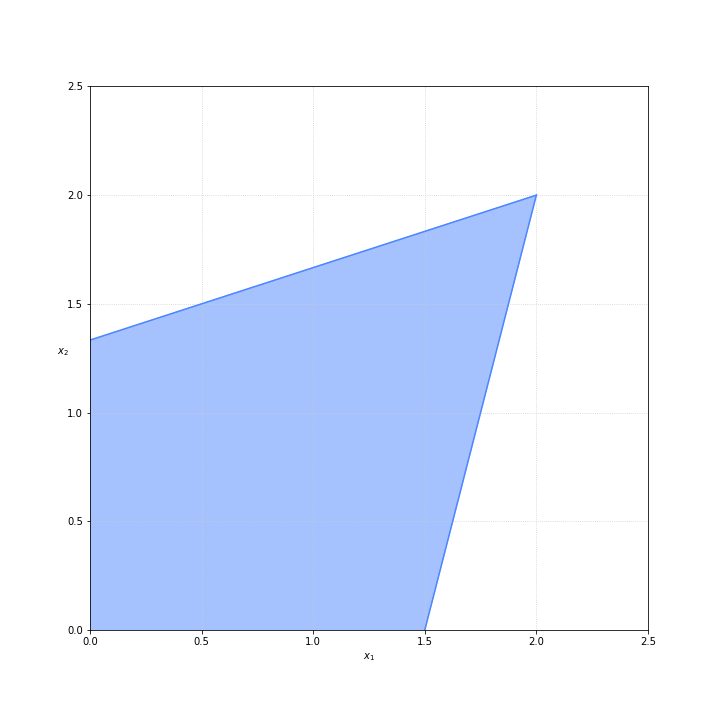
\includegraphics[width=0.5\textwidth]{img/ex1.png}   
    \caption{Přípustná množina řešení k úloze~\ref{eq:P1}.}
    \label{fig:ex1}
\end{figure}

\section{Dualita}
Úloha \ref{eq:LP-P} se nazývá \textbf{primární úloha}. Ke každé primární úloze můžeme přiřadit příslušnou \textbf{duální úlohu}. Je to opět úloha lineárního programování, která pro případ \ref{eq:LP-P} je ve tvaru:
\begin{equation}\tag{LP-D}
    \min \left\{ b^T y \mid A^T y \geq c, y \geq 0 \right\}.
    \label{eq:LP-D}
\end{equation}

\begin{pr}
Duální úloha k úloze \ref{eq:P1} je ve tvaru:
\begin{equation}\tag{P2}
    \begin{split}
        \min 4 y_1 + 6 y_2  & \\
        - y_1 + 4 y_2       &\geq 1 \\
        3 y_1 -   y_2       &\geq 1 \\
        y &\geq 0.
    \end{split}
    \label{eq:P2}
\end{equation}

Přípustná množina řešení je zobrazena na obrázku~\ref{fig:ex2}. Řešením úlohy je vektor $y^* \approx (0.4546, 0.3636)$ s cenou $4$. Implementace v softwaru MOSEK: \url{https://github.com/c0n73x7/D1PL0MK4/blob/master/mosek/ex2.py}.
\end{pr}

\begin{figure}[h!]
    \centering
    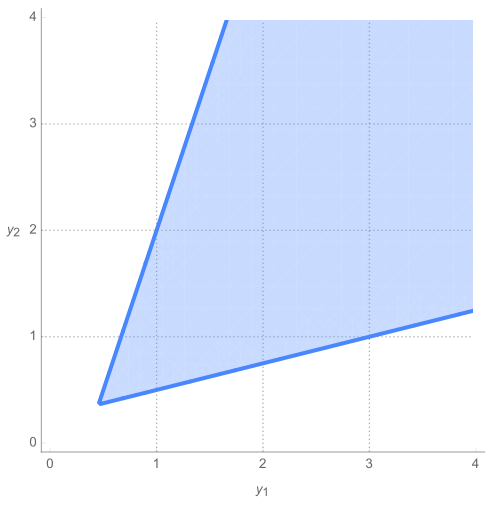
\includegraphics[width=0.5\textwidth]{img/ex2.png}   
    \caption{Přípustná množina řešení k úloze~\ref{eq:P2}.}
    \label{fig:ex2}
\end{figure}

Všimněme si, že v příkladech \ref{eq:P1} a \ref{eq:P2} mají řešení $x^*$ i $y^*$ stejnou cenu. To není náhoda a tento fakt je obsahem silné věty o dualitě, kterou dokázala skupina kolem Alberta W. Tuckera v roce 1948. Začneme slabou větou o dualitě.

\begin{vt}[Slabá o dualitě]
    Nechť $\tilde{x}$ je přípustné řešení \ref{eq:LP-P} a $\tilde{y}$ je přípustné řešení \ref{eq:LP-D}. Potom $c^T \tilde{x} \leq b^T \tilde{y}$.
\end{vt}

Tedy každé přípustné řešení $\tilde{y}$ duální úlohy \ref{eq:LP-D} nám dává horní odhad na maximum účelové funkce primární úlohy \ref{eq:LP-P}. Graficky můžeme slabou větu o dualitě interpretovat jako na obrázku~\ref{fig:weak_duality}. Zatím tedy nevíme, zda vždy existují přípustná (optimální) řešení $x^*$ pro úlohu \ref{eq:LP-P} a $y^*$ pro úlohu \ref{eq:LP-D}, pro která platí $c^T x^* = b^T y^*$. Kladnou odpověď dostaneme z již zmíněné silné věty od dualitě.

\begin{figure}[h!]
    \centering
    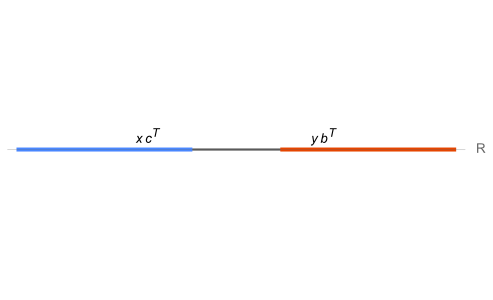
\includegraphics[width=0.5\textwidth]{img/weak_duality.png}   
    \caption{Slabá věta o dualitě.}
    \label{fig:weak_duality}
\end{figure}

\begin{vt}[Silná o dualitě]
    Jestliže úlohy \ref{eq:LP-P} a \ref{eq:LP-D} mají přípustná řešení. Potom
    $$
        \max \left\{ c^T x \mid Ax \leq b, x \geq 0 \right\} = \min \left\{ b^T y \mid A^T y \geq c, y \geq 0 \right\}.
    $$ 
\end{vt}

\section{Komplementární skluzovost}